\documentclass[11pt,a4paper]{article}
\usepackage{fontspec}
\setmainfont{Source Serif 4}[Path=/home/claude/ref/fonts/, UprightFont=SourceSerif4-Regular.ttf, BoldFont=SourceSerif4-Semibold.ttf, ItalicFont=SourceSerif4-It.ttf]
\setmonofont{IBM Plex Mono}[Path=/home/claude/ref/fonts/, UprightFont=IBMPlexMono-Regular.ttf, BoldFont=IBMPlexMono-Medium.ttf, Scale=0.88]
\usepackage[a4paper,margin=2.4cm]{geometry}
\usepackage{amsmath}
\usepackage{graphicx,booktabs,float,caption,array,xcolor,longtable}
\usepackage{xurl}
\usepackage[hidelinks]{hyperref}
\usepackage[round]{natbib}
\usepackage{setspace}
\setstretch{1.08}
\renewcommand{\topfraction}{0.9}
\renewcommand{\bottomfraction}{0.8}
\renewcommand{\textfraction}{0.1}
\renewcommand{\floatpagefraction}{0.75}
\setlength{\parindent}{0pt}
\setlength{\parskip}{0.55em}
\captionsetup{font=small,labelfont=bf}
\setlength{\bibsep}{3pt}
\urlstyle{same}
\hypersetup{pdftitle={Does the 1974 Border Still Show?},pdfauthor={Dr Tristan Hotham}}

\begin{document}
\begin{center}
{\Large\bfseries Does the 1974 Border Still Show? Historic and Modern County Names in the Business Landscape of Lancashire and Yorkshire\par}
\vspace{1.2em}
{\large Dr Tristan Hotham\par}
\vspace{0.3em}
{\small Independent researcher\\
ORCID: 0000-0003-4931-9349\\
DOI: https://doi.org/10.5281/zenodo.24104647\par}
\vspace{0.8em}
2026
\end{center}

\begin{quote}
\small
\begin{center}\textbf{Abstract}\end{center}
The 1974 reorganisation of English local government moved places across the old border between Lancashire and Yorkshire and took large parts of historic Lancashire into new metropolitan counties and Cumbria. Do businesses, clubs and societies now name themselves after the historic county or the one that replaced it? I assemble every OpenStreetMap feature in the region whose name contains Lancashire, Lancs, Yorkshire or Yorks, remove roads, transport and other non-business names, and set aside chains and public bodies, leaving 389 private features. Rates are per 1,000 named business points of interest, following a plan written before any outcome was computed by area. Where the historic border did not move, it remains a sharp naming boundary: within 25 km, 98.3\% of county names on the Yorkshire side say Yorkshire and 2.8\% on the Lancashire side, with no comparable jump at false lines. The pre-specified primary test, in Bowland and West Craven, cannot be answered: the area has no county-named private feature, and too few businesses for that to be informative. In secondary comparisons, the Lancashire name persists in the historic Lancashire parts of the metropolitan counties at about a quarter of its rate inside Lancashire (rate ratio 0.27 in Greater Manchester, 95\% CI 0.15 to 0.48), while their never-Lancashire parts have none; Furness and Cartmel, and Warrington and Widnes, have none. In a pooled model, Lancashire names are associated with both the historic county (rate ratio 15.8) and the county today (4.5). The design is descriptive.

\textbf{Keywords:} historic counties; local government reorganisation; regional identity; place branding; business names; OpenStreetMap; Lancashire; Yorkshire
\end{quote}

\section{Introduction}
On 1 April 1974 the Local Government Act 1972 \citep{lga1972} replaced the administrative counties of England with a new set of metropolitan and non-metropolitan counties. In the north west the changes were large. Lancashire lost Liverpool and its hinterland to Merseyside, Manchester and the cotton towns to Greater Manchester, Furness and Cartmel to the new county of Cumbria, and Warrington and Widnes to Cheshire. It gained the Bowland Rural District, Barnoldswick and Earby from the West Riding of Yorkshire. Saddleworth, also in the West Riding, went to Greater Manchester, and the Sedbergh Rural District to Cumbria. Some of these changes followed the recommendations of the Royal Commission on Local Government in England \citep{rc1969}; others were the government's own.

The reorganisation changed the map of administration, not, its defenders and critics agreed, the map of loyalty. A question in the House of Commons in the year of the change asked whether old county boundary signs could be kept \citep{hansard1974}, and four decades later a government department marked a day for ``England's traditional counties'', describing them as ``fundamental to our culture'' \citep{dclg2013}. Campaigners have argued for the historic counties to stay in public use, and the Historic Counties Trust has digitised their borders \citep{hcbp2024}. For Lancashire and Yorkshire, neighbours with a long sporting and cultural rivalry, the question of which county a place belongs to is not only administrative.

This paper asks whether the 1974 border still shows in one everyday, public and countable form of identity: the names that businesses, clubs and societies give themselves. A shop that calls itself ``Lancashire'' or ``Yorkshire'' makes a small public claim about where it is and whom it serves. If the historic counties remain the frame of local identity, names near the moved lines should follow the historic county; if the new counties have been absorbed, names should follow the new ones; if county naming simply fades where a place left a county, both would be absent.

I use OpenStreetMap, the volunteered world map \citep{goodchild2007,haklay2010}, to collect every feature in and around the two counties whose name contains Lancashire, Lancs, Yorkshire or Yorks, and the vector tiles of OpenFreeMap to count named businesses and venues as a denominator. The design, fixed in a written plan before any share or rate was computed by area, compares zones defined by crossing the historic counties with the counties since 1974: places that stayed in their county, places that moved, and neighbouring places that were never in the county concerned.

There are three findings. First, where the historic border did not move, it remains a sharp naming boundary: almost every county name on one side says Yorkshire and almost every one on the other says Lancashire, and false lines drawn 10 km into either county show no comparable change. Second, the planned primary test, whether businesses in Bowland and West Craven say Yorkshire or Lancashire, cannot be answered from this source: the area has no county-named private feature at all, and its small number of businesses means that even the Yorkshire rate would predict only one or two. Third, in the larger areas that left Lancashire, the Lancashire name has thinned but not vanished in the metropolitan counties, where it survives at about a quarter of its rate inside today's Lancashire, against none in the parts of the same counties that were historically Cheshire; in Furness and Cartmel and in Warrington and Widnes, no Lancashire-named business was found.

The contribution is a transparent, reproducible measurement of historic county identity in the commercial landscape, built from open data, with an explicit accounting of what the data can and cannot show. Section~\ref{sec:lit} reviews work on regional identity and administrative change, vernacular regions measured through names, and place branding. Section~\ref{sec:data} describes the data and Section~\ref{sec:design} the pre-specified design. Section~\ref{sec:results} reports the results, Section~\ref{sec:robust} the checks, and Section~\ref{sec:disc} discusses the findings and their limits.

\section{Background and literature}\label{sec:lit}
\subsection{Regions, institutions and identity after reform}
Geographers have long treated regions as historically contingent institutions rather than fixed containers. In \citet{paasi1986}'s account, a region becomes institutionalised through four stages: it acquires a territorial shape, a symbolic shape, institutions, and an established place in the regional system and in social consciousness. The order of these stages varies, and they can unwind. \citet{paasi2003} later distinguished the identity of a region, the features that mark it off from others, from the regional identity or consciousness of its inhabitants, and argued that both are produced and reproduced in practice. \citet{jones2004} distinguished regional spaces, the territories of economic and political administration, from spaces of regionalism, the cultural and political mobilisations that claim them, using the English South West to show how the two overlap unevenly.

These ideas matter when administration and identity are pulled apart. Studies of municipal amalgamation in Finland describe the deinstitutionalisation of regions and the resistance identities that can follow \citep{zimmerbauer2013}. Focus groups in former Finnish regions found that regions keep their hold on people and things, a ``stickiness'' that persists after official status is lost, so that deinstitutionalised regions survive in a penumbral form \citep{zimmerbauer2017}. In the Netherlands, \citet{terlouw2016,terlouw2018} found that amalgamations remove the identities that held merged communities together and can turn older local identities inward, into resistance identities emphasising historical roots. England's 1974 reform is a case of this kind: county administration moved, while the historic counties kept their names, their cricket clubs and, for many residents, their meaning.

In northern England, county and regional identities have also become political. \citet{giovannini2016} documents the rise of a Yorkshire regionalist party after 2014, drawing on a membership survey, and argues that regional identity and territorial divisions matter in the debate on northern devolution. Cultural historians describe how the North is imagined in national culture \citep{russell2004} and how northern English speech has carried social meanings \citep{wales2006}. A perceptual dialectology study in northern England found only partial support for the idea that listeners recognise nearby accents better, with the proximity effect depending on contact with the dialect \citep{leach2016}.

\subsection{Vernacular regions measured through names}
A long tradition in cultural geography maps vernacular regions through the names that people and businesses use. \citet{reed1976} used business names to map the American South, and \citet{zelinsky1980} mapped vernacular regions across North America; \citet{ambinakudige2009} revisited ``the South'' and ``Dixie'' with business names from telephone directories and GIS; \citet{liesch2015} showed how business directories can delineate vernacular regions in Michigan; and \citet{sublett2021} traced ``Corn Belt'' as an enterprise-naming custom from the nineteenth century to 2020. Names on the landscape can also carry political identity: \citet{gulley1990} found Confederate nationalism in the county names adopted across the former Confederate states after 1861.

More recently, user-generated content has replaced the telephone directory. \citet{hollenstein2010} used millions of geotagged Flickr tags to delimit city cores, and \citet{gao2017} combined several online sources to extract the vague cognitive regions of Northern and Southern California, finding close agreement with a survey of residents. OpenStreetMap is a natural successor: it is open, global and attribute-rich, though its quality varies with the attention of volunteers \citep{goodchild2007,haklay2010}.

\subsection{Place names as brands}
Business names are also marketing. The place-branding literature argues that places are branded through images and associations that residents, firms and administrators produce \citep{kavaratzis2004,kavaratzis2005}, and that brands take part of their meaning from geographical origins \citep{pike2015}. A ``Yorkshire'' tea room or ``Lancashire'' builder borrows the associations of the county name, so naming reflects both identity and a judgement about what customers will recognise. This matters for interpretation: a name can follow the market rather than the founder's sense of belonging.

\subsection{Borders as discontinuities}
A final literature treats historical borders as natural experiments. Geographic regression discontinuity designs compare places just either side of a boundary \citep{keele2015}. \citet{dell2010} used the boundary of Peru's colonial mining labour system to show long-run effects on consumption and stunting, and \citet{becker2016} showed that communities on the former Habsburg side of a long-gone border still trust courts and police more. \citet{falck2012} found that historical dialect similarity predicts migration between German regions. These studies show that dissolved borders can persist in behaviour; the present study asks whether a moved English county border persists in naming, with a design that is descriptive rather than causal.

\subsection{What is new here}
Studies of the 1974 reorganisation have concentrated on its administrative design. Work on regional identity after reform has relied on interviews, focus groups and documents. The vernacular-region tradition has measured names, but mostly in the United States and without a moved boundary to test against. This paper brings the three together: it measures county names in open data across a border that moved, with zones that separate the historic county from the county today, a denominator for business density, and a plan fixed before the outcome was examined.

\section{Data}\label{sec:data}
\subsection{County-named features}
The names come from an OpenStreetMap extract \citep{osm2026} queried through QLever in 2026: every UK feature whose name contains Lancashire, Lancs, Yorkshire, Yorks, Red Rose, White Rose or one of several early kingdom names, with its shop, amenity, office, craft, leisure and highway tags and its geometry. The file has 7,500 rows; 2,693 contain a Lancashire, Yorkshire or rose word as a whole word. Each feature is located at its node or at a representative point of its geometry.

Names were classified by fixed rules (Appendix Table~\ref{tab:flow}). Lancashire names match \texttt{lancashire}, \texttt{lancs} or \texttt{lancastrian}; Yorkshire names match \texttt{yorkshire} or \texttt{yorks}; 10 names with both words were excluded. ``Red Rose'' and ``White Rose'', the counties' emblems, are also common pub and flower names, so they are used only in a sensitivity check. Roads and bus stops (highway tags), untagged line features (railways, canals, paths), names in which the county word is part of a street name (``Yorkshire Street Dental''), and product or breed names (``Yorkshire pudding'') were dropped. Each kept feature was typed as private (businesses, clubs, societies and venues), public (police, councils, NHS bodies, schools, colleges, universities, utilities, armed forces and regional broadcasters), or chain (the same normalised name at three or more places more than 1 km apart, such as the branches of a building society, whose names say where the firm began rather than where the branch is). The same name within 300 m was treated as one feature.

Every kept feature within 40 km of the historic Lancashire and Yorkshire line, and every feature in a zone that moved, was read by eye on a list without zone or distance columns. 75 hand decisions are recorded in \texttt{code/overrides.csv}: bus routes and stops held as relations, long-distance paths, administrative boundary relations, car parks, memorials, a duplicated golf club, a surname (a car dealer named after its founders), and type corrections such as private hospitals and schools that the public-body rule had caught. The main sample is 389 private features with a county word in the study zones: 77 Lancashire and 312 Yorkshire.

\subsection{Boundaries and zones}
Historic counties come from the Historic County Borders Project \citep{hcbp2024}, UK Definition A, digitised from Ordnance Survey first edition maps. The counties since 1974 are today's ceremonial counties built from the ONS December 2023 local authority districts \citep{ons2023}. For this region the ceremonial counties follow the 1974 lines, except that Cleveland and Humberside, which existed from 1974 to 1996, have since been dissolved; Stockton-on-Tees, which is split by the Tees, takes its historic county on each bank. Crossing the two maps gives zones (Table~\ref{tab:zones}). Pieces smaller than 5 km$^2$ were treated as slivers from the two sources' different line work; no feature in the main sample fell in a sliver where the two disagree.

The areas moved in 1974 recovered in this way are Bowland and West Craven, from Yorkshire to Lancashire (385 km$^2$); Saddleworth, to Greater Manchester (76 km$^2$); Sedbergh and Dent, to Cumbria (213 km$^2$); south Teesdale, to Durham (392 km$^2$); and, from Lancashire, Furness and Cartmel to Cumbria (621 km$^2$), the Warrington and Widnes area to Cheshire (147 km$^2$), and large areas to Greater Manchester (929 km$^2$) and Merseyside (489 km$^2$). The metropolitan counties also took historic Cheshire: Stockport, Sale, Altrincham and Hyde in Greater Manchester (254 km$^2$) and the Wirral in Merseyside (157 km$^2$). A small part of historic Lancashire around Walsden had already passed into Yorkshire before 1974 and is reported separately. Two lines are measured: the historic border between Lancashire and Yorkshire, and the border between the Yorkshire ceremonial counties and Lancashire, Greater Manchester and Cumbria. Figure~\ref{fig:map} maps both with every main-sample feature.

\begin{figure}[tbp]\centering
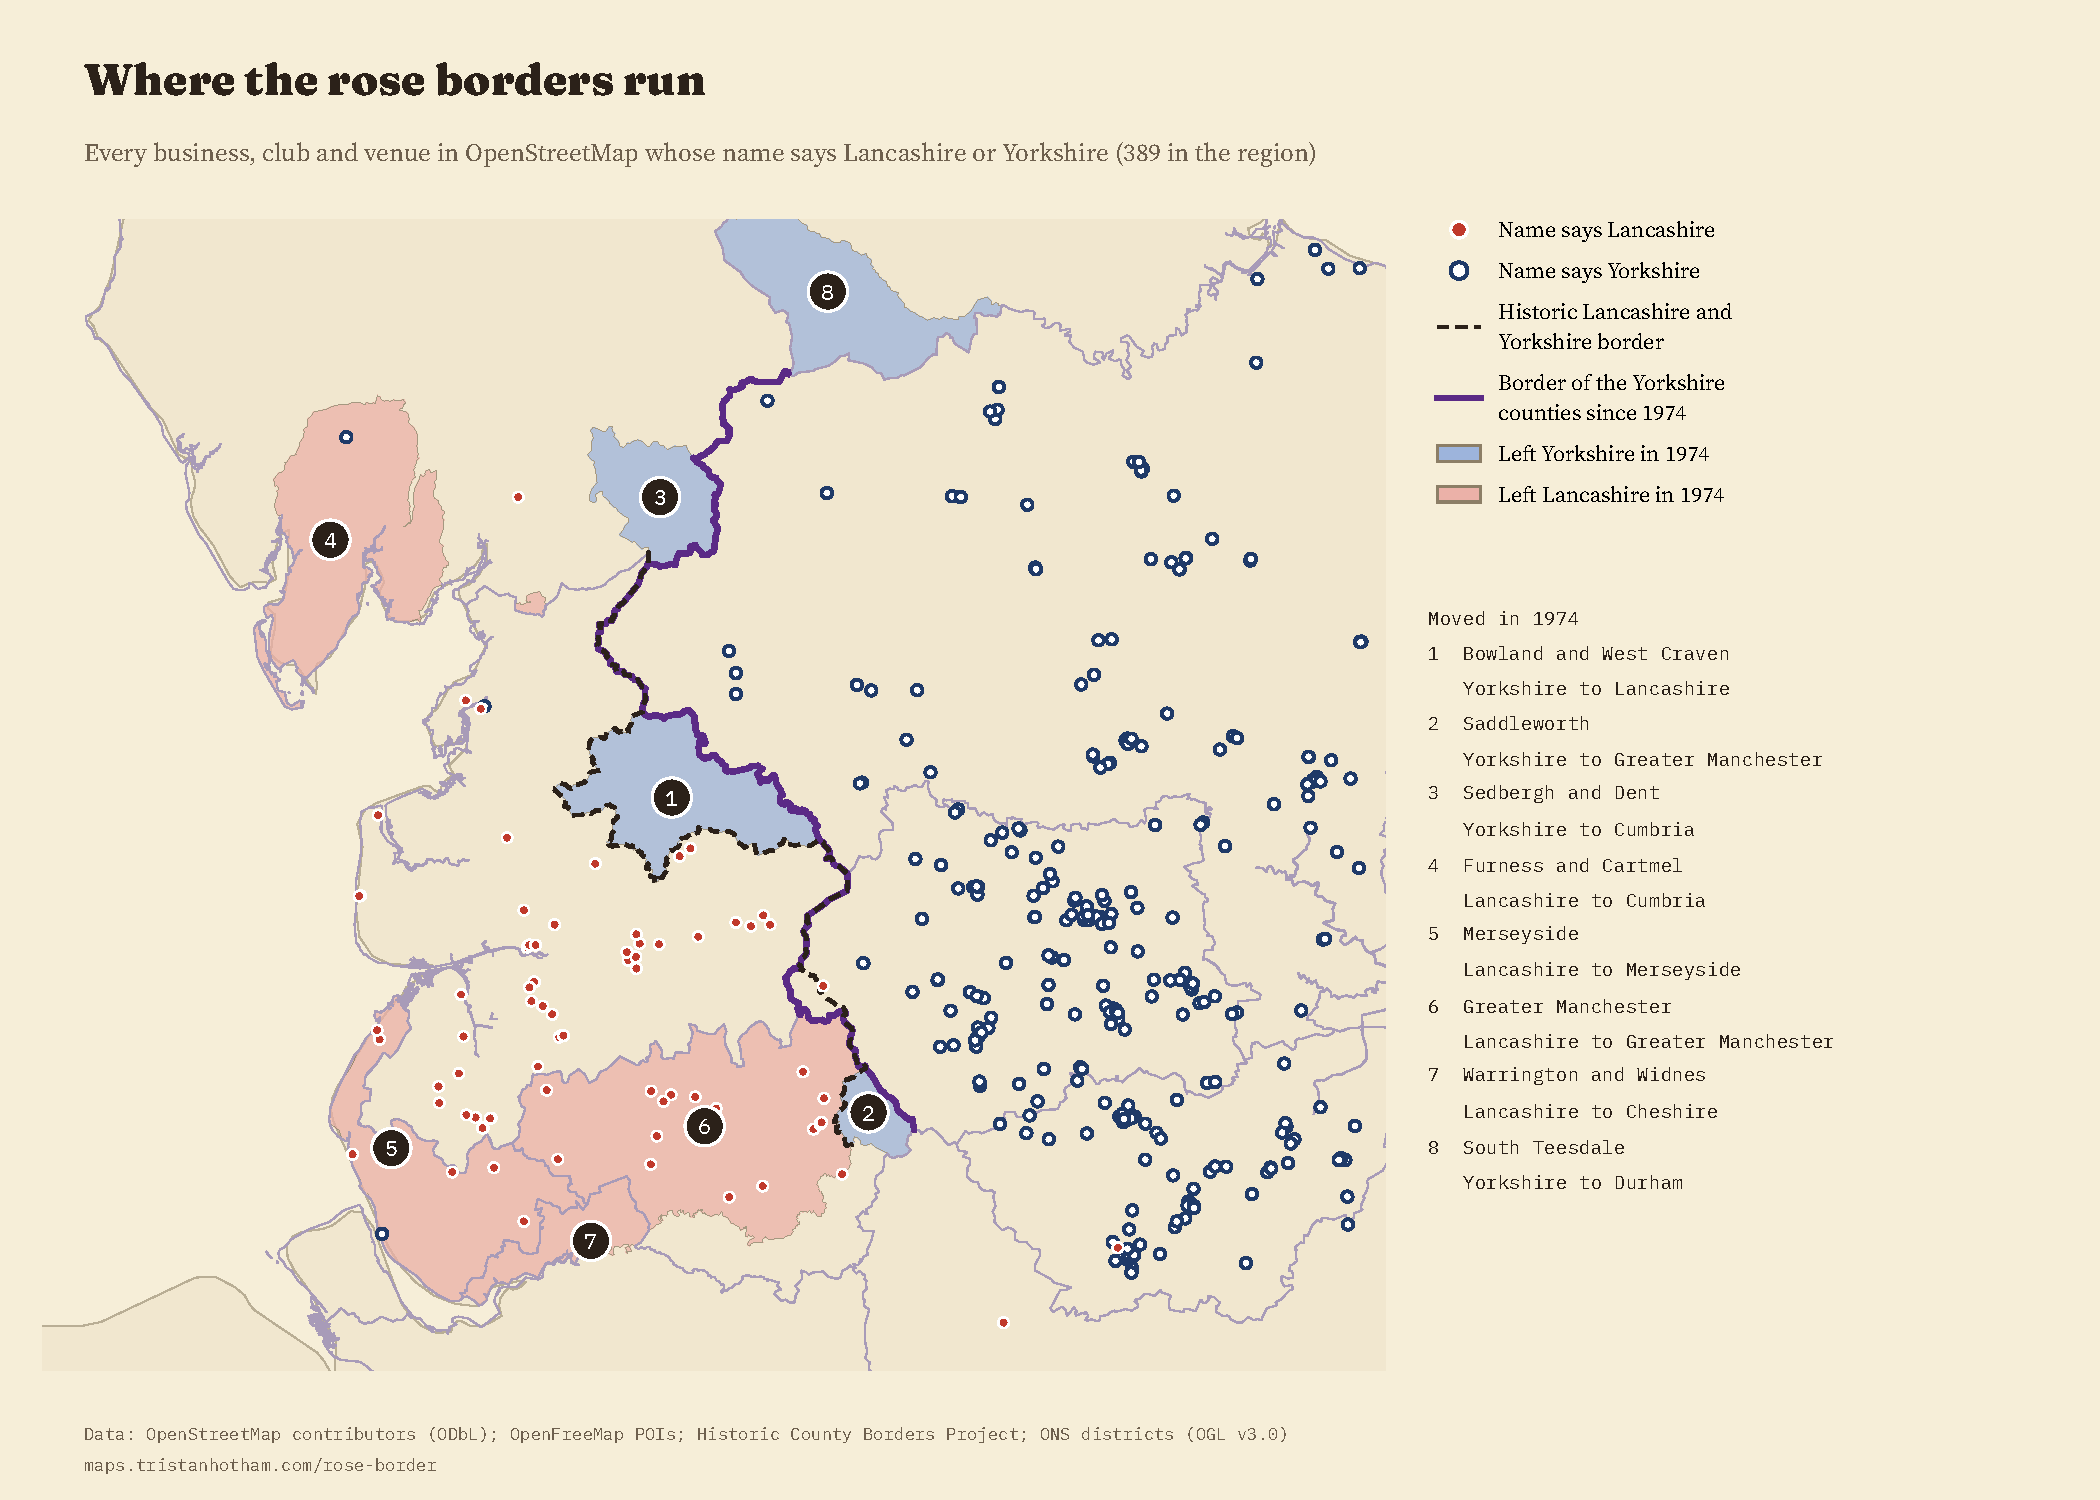
\includegraphics[width=\textwidth]{f_map.pdf}
\caption{County-named private features (main sample), the historic border, the border of the Yorkshire counties since 1974, and the areas moved in 1974 (numbered).}\label{fig:map}
\end{figure}

\begin{table}[tbp]\centering\scriptsize\caption{Zones: historic county crossed with the county since 1974. Area (km$^2$), named business points of interest (OpenFreeMap) and county-named private features (main sample) where the row is used in Table~\ref{tab:rates}. LL and YY counts in Table~\ref{tab:rates} use the bands stated there.}\label{tab:zones}\begin{tabular}{lp{7.2cm}rrrr}\toprule Code & Zone & km$^2$ & POIs & Lancs. & Yorks.\\\midrule
LL & Historic Lancashire, still in Lancashire & 2,679 & 11,968 & 49 & 1\\
YY & Historic Yorkshire, still in a Yorkshire county & 14,598 & 42,080 & 1 & 59\\
T\_YL & Bowland and West Craven: Yorkshire to Lancashire in 1974 & 385 & 223 & 0 & 0\\
T\_YG & Saddleworth: Yorkshire to Greater Manchester & 76 & 174 &  & 0\\
T\_YC & Sedbergh and Dent: Yorkshire to Cumbria & 213 & 80 &  & 0\\
T\_YD & South Teesdale: Yorkshire to Durham & 392 & 57 &  & 0\\
L\_GM & Lancashire to Greater Manchester & 929 & 15,382 & 17 & 0\\
L\_MS & Lancashire to Merseyside & 489 & 6,893 & 6 & \\
L\_CU & Furness and Cartmel: Lancashire to Cumbria & 621 & 1,279 & 0 & \\
L\_CH & Warrington and Widnes: Lancashire to Cheshire & 147 & 1,482 & 0 & \\
C\_GM & Historic Cheshire in Greater Manchester & 254 & 3,189 & 0 & \\
C\_MS & Historic Cheshire in Merseyside (Wirral) & 157 & 1,691 & 0 & \\
CC & Historic Cheshire, still in Cheshire & 2,193 & 7,168 & 1 & \\
W\_CU & Historic Westmorland, in Cumbria & 2,032 & 2,380 & 1 & 0\\
U\_CU & Historic Cumberland, in Cumbria & 3,937 & 3,949 & 0 & \\
DD & Historic Durham, still in Durham & 2,290 & 6,960 &  & 0\\
\bottomrule\end{tabular}\end{table}

\subsection{A denominator}
Areas differ in how many businesses they have and in how thoroughly volunteers have mapped them. To express county names as rates, I read every OpenFreeMap vector tile at zoom 14 over the region \citep{openfreemap2026}, 219,501 named points of interest in the study zones, and counted the 106,414 in business and venue classes (shops, food and drink, lodging, offices, leisure), leaving out transport, parking, street furniture and public services. These come from the same OpenStreetMap database as the names and so share its coverage. Rates are county-named private features per 1,000 named business points of interest.

\section{Research design}\label{sec:design}
The analysis plan was written in \texttt{NOTES.md} after the data construction above but before any share or rate was computed by zone or distance. Its elements were as follows.

\textbf{H1 (primary).} In Bowland and West Craven (T\_YL), the share $s_T$ of county-named private features that say Yorkshire lies between the shares in historic Yorkshire that stayed in Yorkshire ($s_Y$) and historic Lancashire that stayed in Lancashire ($s_L$), each within 25 km of the historic line. The persistence index $P=(s_T-s_L)/(s_Y-s_L)$ is 1 if the area names itself like Yorkshire and 0 if like Lancashire, with a cluster bootstrap by 5 km cell; the decision rule was that an interval above 0.5 means the historic county dominates and below 0.5 the modern one. A linear-in-distance model at the line (M1b) was also specified, as a logit with separate slopes each side and errors clustered by 5 km cell.

\textbf{H2 (secondary).} For each county name, the rate per 1,000 business points of interest in each zone, compared by exact conditional rate ratios \citep{clopper1934} with the stayed zone of that historic county (all of LL for the Lancashire name; YY within 25 km for the Yorkshire name), and with a neighbouring benchmark that was never in the county: historic Cheshire in Greater Manchester (C\_GM) for the Lancashire part of Greater Manchester, the Wirral (C\_MS) for Merseyside, Westmorland (W\_CU) for Furness and for Sedbergh, Cheshire (CC) for Warrington and Widnes, historic Lancashire (LL, band) for Bowland, the Lancashire part of Greater Manchester for Saddleworth, and Durham for south Teesdale. Persistence predicts moved zones near their stayed zone; replacement predicts them near the benchmark. A derived index $Q=(r_{moved}-r_{bench})/(r_{stayed}-r_{bench})$ summarises where each lies, with a cluster bootstrap.

\textbf{M2 (pooled).} A Poisson regression of the count of features naming county $N$ in each zone-by-5 km cell unit, with the log of business points of interest as offset, on indicators for being in historic $N$ ($H$) and in modern $N$ ($M$), errors clustered by 20 km block \citep{cameron2015}. For Lancashire, $M$ is ceremonial Lancashire; for Yorkshire, the four Yorkshire ceremonial counties. The two coefficients are identified by units where the maps disagree.

\textbf{H3 (validation).} Public bodies named for a county should follow the modern line.

\textbf{Checks.} Placebo P1: the jump in the Yorkshire share across the historic line where it did not move, against false lines 10 km into each county, in 10 km windows. P2: within Greater Manchester and Merseyside, the Lancashire rate in the historic Lancashire parts against the historic Cheshire parts (rows of H2). Alternatives: bandwidths of 10, 15 and 40 km; chains included (one per name per zone); public bodies included; all types; rose names added; no deduplication; tagged features only; all named points of interest as denominator; clustering by 10 km cell. Leave-one-out: Bowland (Ribble Valley) and West Craven (Pendle) separately. Shares carry Wilson intervals \citep{wilson1927} and counts exact Poisson intervals \citep{garwood1936}. The plan stated what would count against persistence: $P$ below 0.5; no Yorkshire excess in Bowland over the Lancashire band; no Lancashire excess in Furness over Westmorland and Cumberland.

\section{Results}\label{sec:results}
\subsection{The historic line where it did not move}
Along most of its length the 1974 border of the Yorkshire counties follows the historic border, and there the line is a sharp naming boundary (Figure~\ref{fig:profile}). Within 25 km of the historic line, 59 of 60 county-named private features on the Yorkshire side say Yorkshire (98.3\%, 95\% CI 91.1 to 99.7) and 1 of 36 on the Lancashire side (2.8\%, CI 0.5 to 14.2). The logit of M1b could not be estimated because of near-complete separation, which is itself the finding; the linear probability version puts the difference at the line at 78 percentage points (CI 44 to 111; Table~\ref{tab:placebo}).

\begin{figure}[tbp]\centering
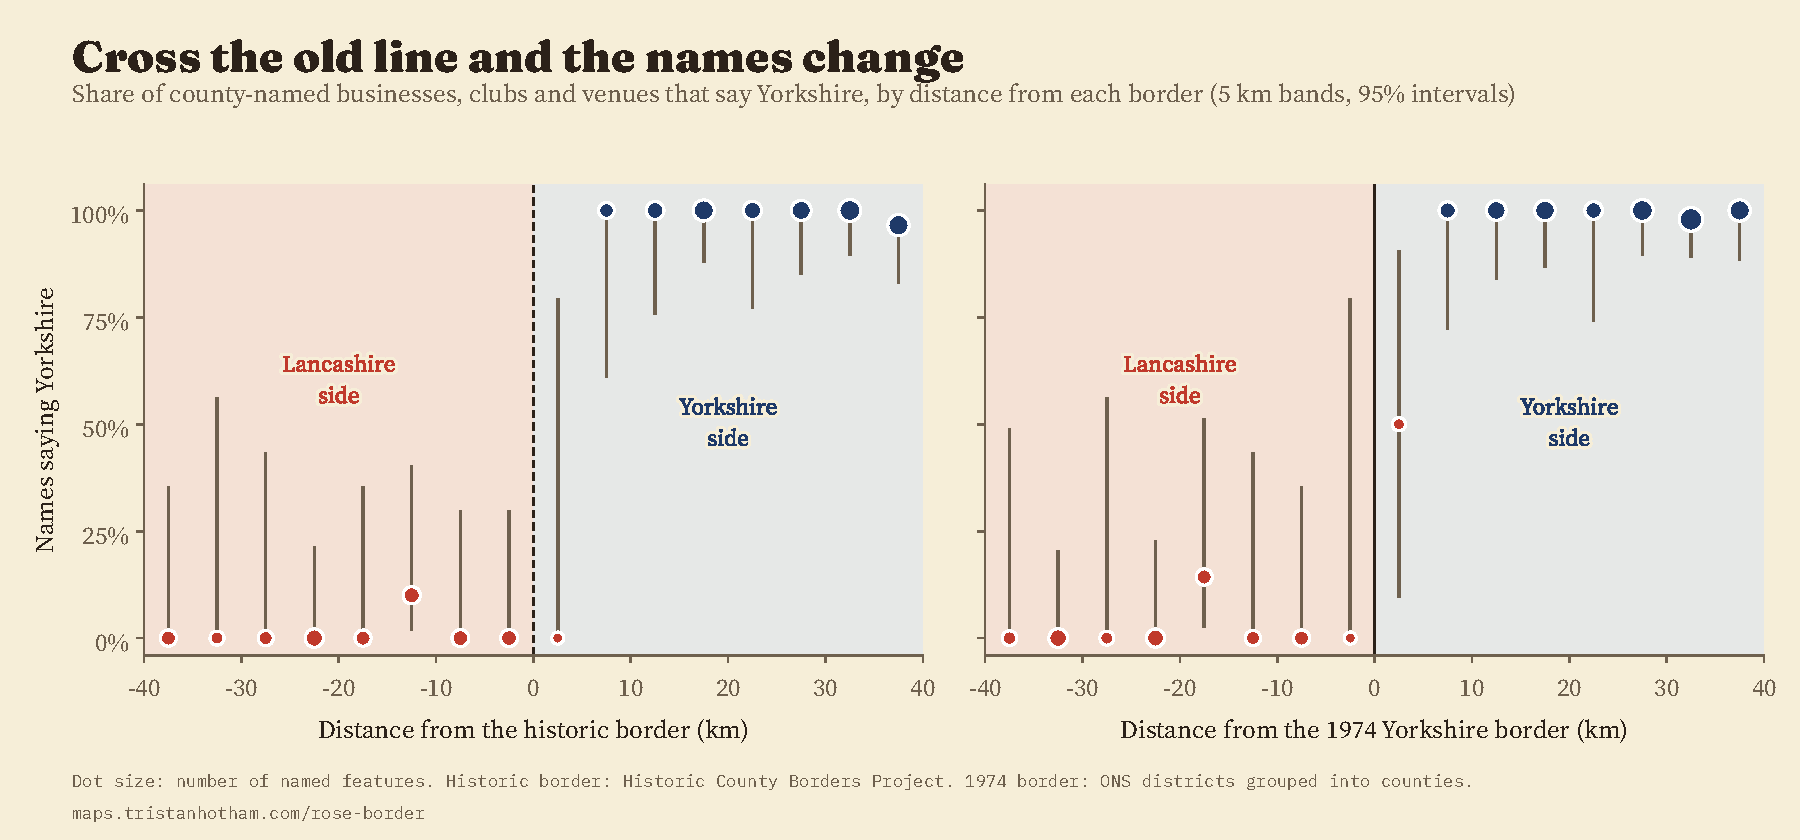
\includegraphics[width=\textwidth]{f_profile.pdf}
\caption{Share of county-named private features naming Yorkshire by signed distance from the historic border (left) and the border of the Yorkshire counties since 1974 (right), 5 km bands, Wilson 95\% intervals.}\label{fig:profile}
\end{figure}

\subsection{H1: Bowland and West Craven}
The primary test cannot be carried out (Table~\ref{tab:shares}). Bowland and West Craven contain no county-named private feature in OpenStreetMap, so $s_T$ and $P$ are undefined. The same is true of Saddleworth, Sedbergh and Dent, and south Teesdale. This is not strong evidence that the Yorkshire name has disappeared there: the four areas have only 534 named business points of interest between them, and at the Yorkshire rate of the band beside the line about 3.7 Yorkshire names would be expected in all four together (Table~\ref{tab:rates}). The upper limits of the rate ratios are correspondingly wide (for Bowland and West Craven, up to 2.5 times the stayed Yorkshire rate). Two county names that are not private do occur in Bowland and West Craven: a branch of a building society named after Yorkshire, a chain, and a water-utility sign in the Forest of Bowland whose wording names Lancashire. By the decision rules of the plan, H1 is unresolved.

\begin{table}[tbp]\centering\footnotesize\caption{H1: county-named private features by zone and the share naming Yorkshire (Wilson 95\% interval).}\label{tab:shares}\begin{tabular}{lrrl}\toprule Zone & Lancashire & Yorkshire & \% Yorkshire [95\% CI]\\\midrule
Historic Lancashire, still Lancashire (within 25 km) & 35 & 1 & 2.8 [0.5, 14.2]\\
Historic Yorkshire, still Yorkshire (within 25 km) & 1 & 59 & 98.3 [91.1, 99.7]\\
Bowland and West Craven (Yorkshire to Lancashire) & 0 & 0 & \\
Saddleworth (Yorkshire to Greater Manchester) & 0 & 0 & \\
Sedbergh and Dent (Yorkshire to Cumbria) & 0 & 0 & \\
South Teesdale (Yorkshire to Durham) & 0 & 0 & \\
Lancashire to Greater Manchester & 17 & 0 & 0.0 [0.0, 18.4]\\
Lancashire to Merseyside & 6 & 1 & 14.3 [2.6, 51.3]\\
Furness and Cartmel (Lancashire to Cumbria) & 0 & 1 & 100.0 [20.7, 100.0]\\
Warrington and Widnes (Lancashire to Cheshire) & 0 & 0 & \\
\midrule Persistence index $P$ for T\_YL & \multicolumn{3}{l}{not estimable (no county-named feature in the moved zone)}\\
\bottomrule\end{tabular}\end{table}

\subsection{H2: areas that left Lancashire}
The secondary comparisons, in the larger areas that left Lancashire, are more informative (Table~\ref{tab:rates}, Figure~\ref{fig:rates}). Inside today's Lancashire there are 4.09 Lancashire-named private features per 1,000 business points of interest (49 features). In the historic Lancashire part of Greater Manchester the rate is 1.11 (17 features), a rate ratio of 0.27 (95\% CI 0.15 to 0.48); in the historic Lancashire part of Merseyside it is 0.87 (6 features; ratio 0.21, CI 0.07 to 0.50). The benchmarks that were never Lancashire have none: the historic Cheshire part of Greater Manchester (3,189 business points of interest) and the Wirral (1,691). Separately, neither ratio against its own benchmark has a lower limit far from 1 (0.86 and 0.29), but pooled, as an exploratory comparison not in the plan, the old Lancashire parts of the two metropolitan counties have 23 Lancashire names and the old Cheshire parts none where 5.0 would be expected at the same rate (exact lower limit of the rate ratio 1.26; $p=0.025$). The persistence index $Q$ places Greater Manchester at 27\% of the way from its benchmark to stayed Lancashire (CI 13 to 55) and Merseyside at 21\% (CI 5 to 51).

\begin{figure}[tbp]\centering
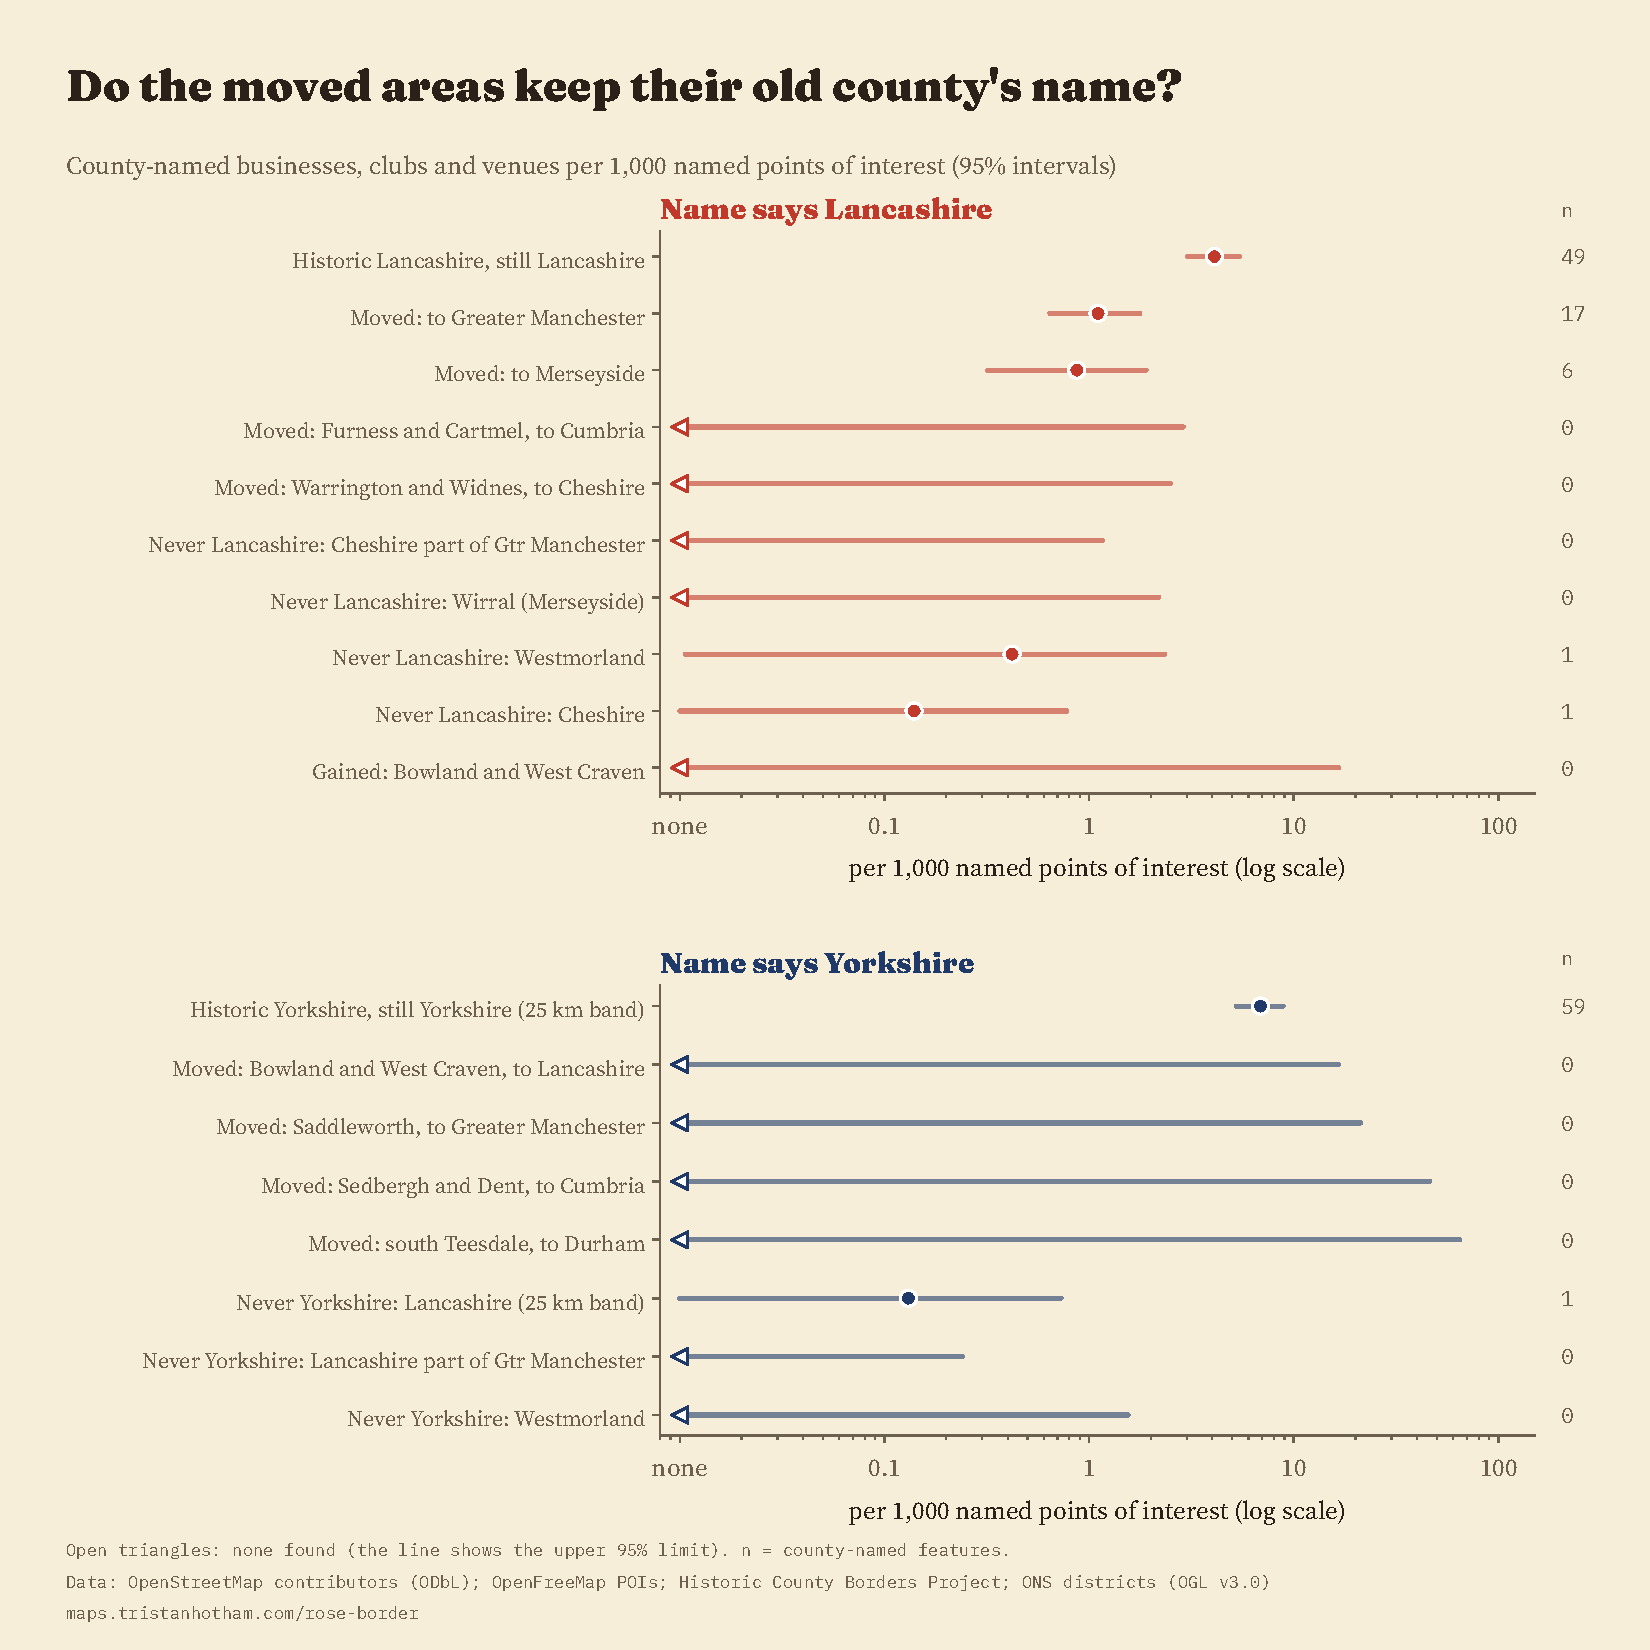
\includegraphics[width=0.92\textwidth]{f_rates.pdf}
\caption{County-named private features per 1,000 named business points of interest by zone, with exact 95\% intervals. Open triangles: none found.}\label{fig:rates}
\end{figure}

In the areas that left Lancashire for the counties beyond it, no Lancashire-named private feature was found. In Furness and Cartmel about 5.2 would be expected at the rate of stayed Lancashire (rate ratio upper limit 0.73), and in Warrington and Widnes about 6.1 (upper limit 0.63). Both are significantly below stayed Lancashire and indistinguishable from their never-Lancashire benchmarks (Westmorland has 1 Lancashire name and Cheshire 1). Figure~\ref{fig:expected} compares found and expected counts for every moved area.

\begin{figure}[tbp]\centering
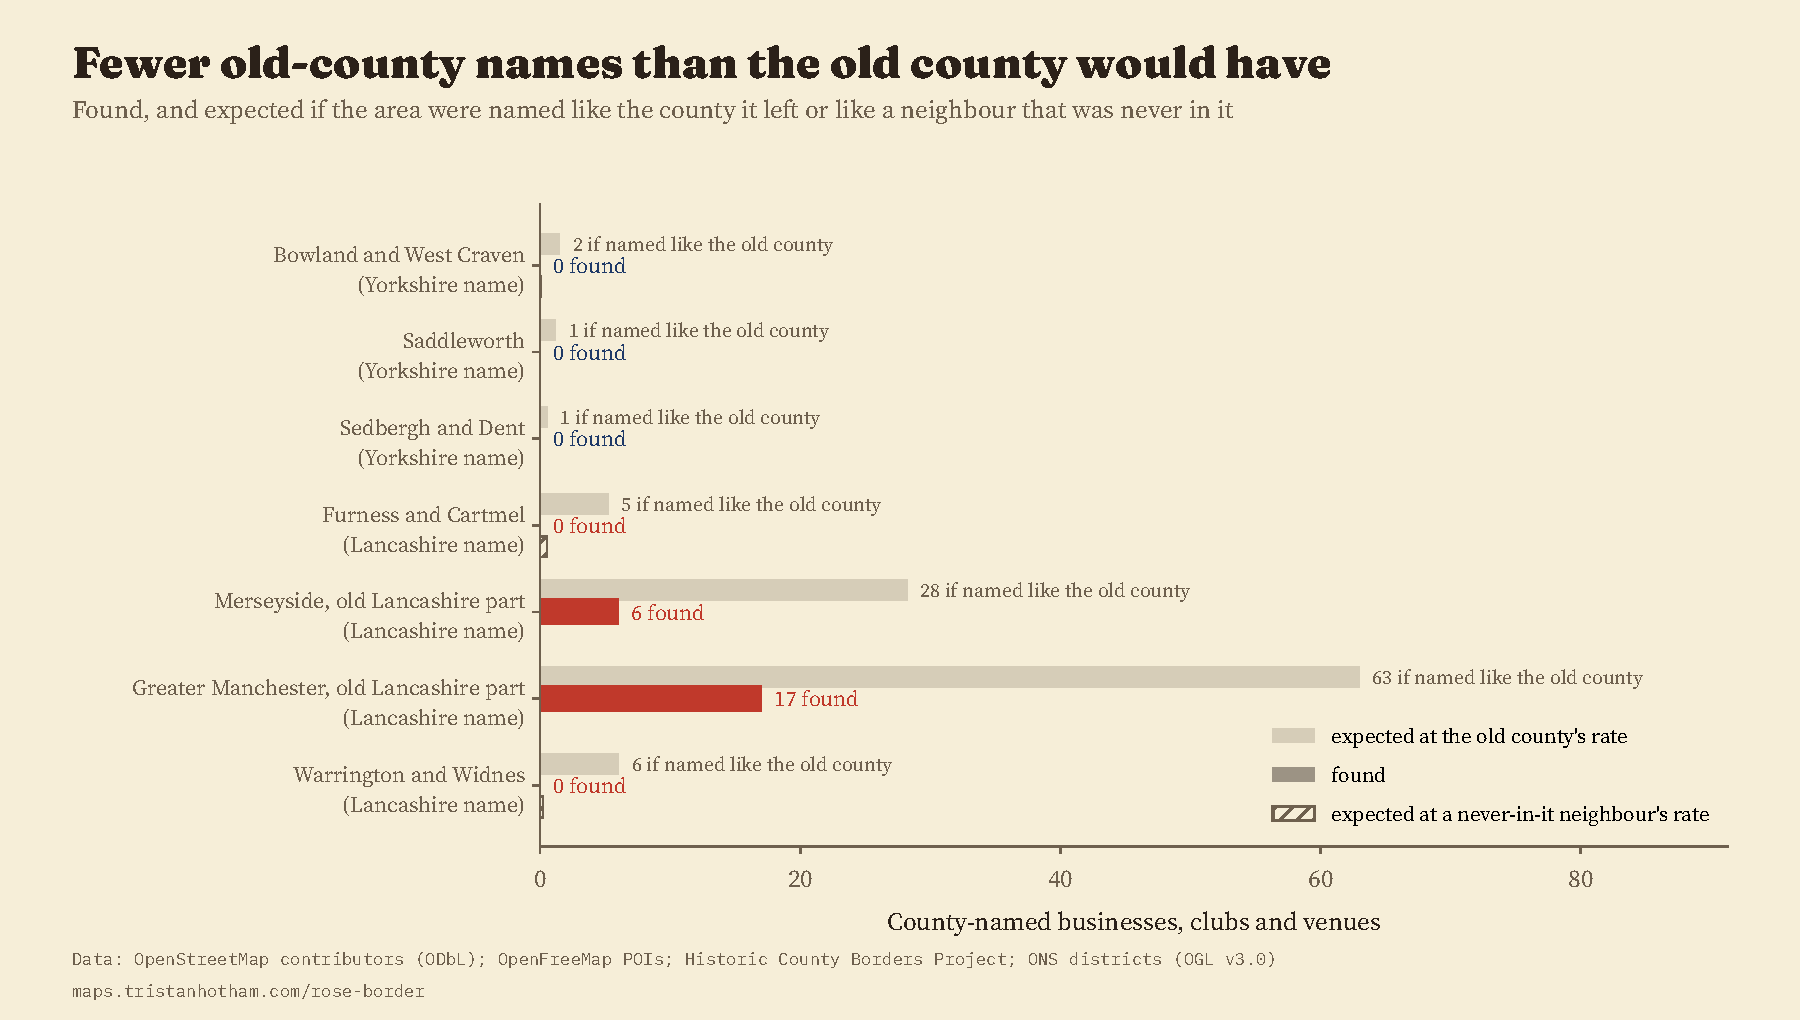
\includegraphics[width=0.92\textwidth]{f_expected.pdf}
\caption{County-named private features found in each moved area, and the numbers expected at the rate of the county it left and at the rate of a never-in-the-county neighbour.}\label{fig:expected}
\end{figure}

\begin{table}[tbp]\centering\scriptsize\caption{H2: county-named private features per 1,000 named business POIs by zone (exact Poisson 95\% CI); rate ratio against the stayed zone of the historic county (LL, all of it, for the Lancashire name; YY within 25 km of the line for the Yorkshire name) with the exact conditional interval; the count expected at the stayed zone's rate; and the rate ratio against the never-in-the-county benchmark named in the text. $\infty$: the comparison zone has none.}\label{tab:rates}\setlength{\tabcolsep}{3pt}\begin{tabular}{lrrllrl}\toprule Zone (role) & $n$ & POIs & Rate [95\% CI] & RR vs stayed & Expected & RR vs benchmark\\\midrule
\multicolumn{7}{l}{\textit{Name says Lancashire}}\\
\quad LL (stayed) & 49 & 11,968 & 4.09 [3.03, 5.41] &  &  & \\
\quad L\_GM (moved) & 17 & 15,382 & 1.11 [0.64, 1.77] & 0.27 [0.15, 0.48] & 63.0 & \\
\quad L\_MS (moved) & 6 & 6,893 & 0.87 [0.32, 1.89] & 0.21 [0.07, 0.50] & 28.2 & \\
\quad L\_CU (moved) & 0 & 1,279 & 0.00 [0.00, 2.88] & 0.00 [0.00, 0.73] & 5.2 & 0.00 [0.00, 72.57]\\
\quad L\_CH (moved) & 0 & 1,482 & 0.00 [0.00, 2.49] & 0.00 [0.00, 0.63] & 6.1 & 0.00 [0.00, 188.63]\\
\quad L\_YO (moved) & 0 & 75 & 0.00 [0.00, 49.19] & 0.00 [0.00, 12.48] & 0.3 & 0.00 [0.00, 4461.60]\\
\quad C\_GM (benchmark) & 0 & 3,189 & 0.00 [0.00, 1.16] & 0.00 [0.00, 0.29] & 13.1 & \\
\quad C\_MS (benchmark) & 0 & 1,691 & 0.00 [0.00, 2.18] & 0.00 [0.00, 0.55] & 6.9 & \\
\quad CC (benchmark) & 1 & 7,168 & 0.14 [0.00, 0.78] & 0.03 [0.00, 0.20] & 29.3 & \\
\quad W\_CU (benchmark) & 1 & 2,380 & 0.42 [0.01, 2.34] & 0.10 [0.00, 0.60] & 9.7 & \\
\quad U\_CU (benchmark) & 0 & 3,949 & 0.00 [0.00, 0.93] & 0.00 [0.00, 0.24] & 16.2 & \\
\quad YY (benchmark) & 1 & 8,580 & 0.12 [0.00, 0.65] & 0.03 [0.00, 0.17] & 35.1 & \\
\quad T\_YL (gained) & 0 & 223 & 0.00 [0.00, 16.54] & 0.00 [0.00, 4.20] & 0.9 & 0.00 [0.00, 1500.54]\\
\multicolumn{7}{l}{\textit{Name says Yorkshire}}\\
\quad YY (stayed) & 59 & 8,580 & 6.88 [5.23, 8.87] &  &  & \\
\quad T\_YL (moved) & 0 & 223 & 0.00 [0.00, 16.54] & 0.00 [0.00, 2.48] & 1.5 & 0.00 [0.00, 1336.32]\\
\quad T\_YG (moved) & 0 & 174 & 0.00 [0.00, 21.20] & 0.00 [0.00, 3.18] & 1.2 & \\
\quad T\_YC (moved) & 0 & 80 & 0.00 [0.00, 46.11] & 0.00 [0.00, 6.92] & 0.6 & \\
\quad T\_YD (moved) & 0 & 57 & 0.00 [0.00, 64.72] & 0.00 [0.00, 9.71] & 0.4 & \\
\quad LL (benchmark) & 1 & 7,641 & 0.13 [0.00, 0.73] & 0.02 [0.00, 0.11] & 52.5 & \\
\quad L\_GM (benchmark) & 0 & 15,382 & 0.00 [0.00, 0.24] & 0.00 [0.00, 0.04] & 105.8 & \\
\quad W\_CU (benchmark) & 0 & 2,380 & 0.00 [0.00, 1.55] & 0.00 [0.00, 0.23] & 16.4 & \\
\quad DD (benchmark) & 0 & 6,960 & 0.00 [0.00, 0.53] & 0.00 [0.00, 0.08] & 47.9 & \\
\quad L\_YO (gained) & 0 & 75 & 0.00 [0.00, 49.19] & 0.00 [0.00, 7.38] & 0.5 & 0.00 [0.00, 3973.32]\\
\bottomrule\end{tabular}\end{table}

\subsection{M2: both maps at once}
The pooled Poisson model (Table~\ref{tab:m2}) summarises the pattern. For the Lancashire name, being in historic Lancashire multiplies the rate by 15.8 (95\% CI 5.6 to 44.6) holding the county today fixed, and being in today's Lancashire by 4.5 (CI 2.1 to 9.3) holding the historic county fixed. The historic coefficient is identified by the large areas of historic Lancashire now in Greater Manchester, Merseyside, Cumbria and Cheshire (142 units); the modern one by the comparison of those areas with stayed Lancashire and by Bowland and West Craven (18 units). For the Yorkshire name the model returns 4.7 for the historic county and 33.5 for the county today, but every unit where the two maps disagree has a count of zero and the disagreeing units are small, so the split between the two is weakly identified; it reverses when chain branches are counted (Section~\ref{sec:robust}).

\begin{table}[tbp]\centering\footnotesize\caption{M2: Poisson regression of county-named private features on indicators for the historic county and the county today, with log named business POIs as offset; units are 5 km cells within zones; standard errors clustered by 20 km block.}\label{tab:m2}\begin{tabular}{llrrlr}\toprule Name & Indicator & $b$ & (SE) & Rate ratio [95\% CI] & $p$\\\midrule
Lancashire & historic county & 2.758 & (0.530) & 15.78 [5.58, 44.57] & 0.0000\\
Lancashire & county today & 1.494 & (0.378) & 4.45 [2.12, 9.34] & 0.0001\\
& \multicolumn{5}{p{11cm}}{units 1,390; features 76; clusters 105; units where the two disagree: historic only 142, today only 18}\\\midrule
Yorkshire & historic county & 1.549 & (0.635) & 4.71 [1.36, 16.33] & 0.0147\\
Yorkshire & county today & 3.512 & (0.628) & 33.50 [9.78, 114.76] & 0.0000\\
& \multicolumn{5}{p{11cm}}{units 1,390; features 310; clusters 105; units where the two disagree: historic only 44, today only 4}\\\bottomrule\end{tabular}\end{table}

\subsection{H3: public bodies}
County-named public bodies and chain branches in the moved zones are few (13). Most are branches of a building society named after Yorkshire, in Greater Manchester, Merseyside, Warrington and West Craven, which say nothing about local identity. The others are a water-utility sign in Bowland naming Lancashire, a probation company in Furness named after both Cumbria and Lancashire, and a mining museum in Greater Manchester named after Lancashire. The validation test therefore has too few cases to evaluate; the three cases are consistent with public names following the modern county (Bowland, Furness) or with heritage institutions keeping the historic one (the museum).

\section{Robustness}\label{sec:robust}
\textbf{Placebo lines.} Across the historic line where it did not move, the share naming Yorkshire jumps by 86 points within 10 km windows (CI 50 to 100). At a false line 10 km inside Lancashire the change is $-$8 points (CI $-$23 to 0), and at a false line 10 km inside Yorkshire 14 points (CI 0 to 60) (Table~\ref{tab:placebo}, Figure~\ref{fig:placebo}). The samples in the windows are small, which is why the intervals are wide.

\begin{figure}[tbp]\centering
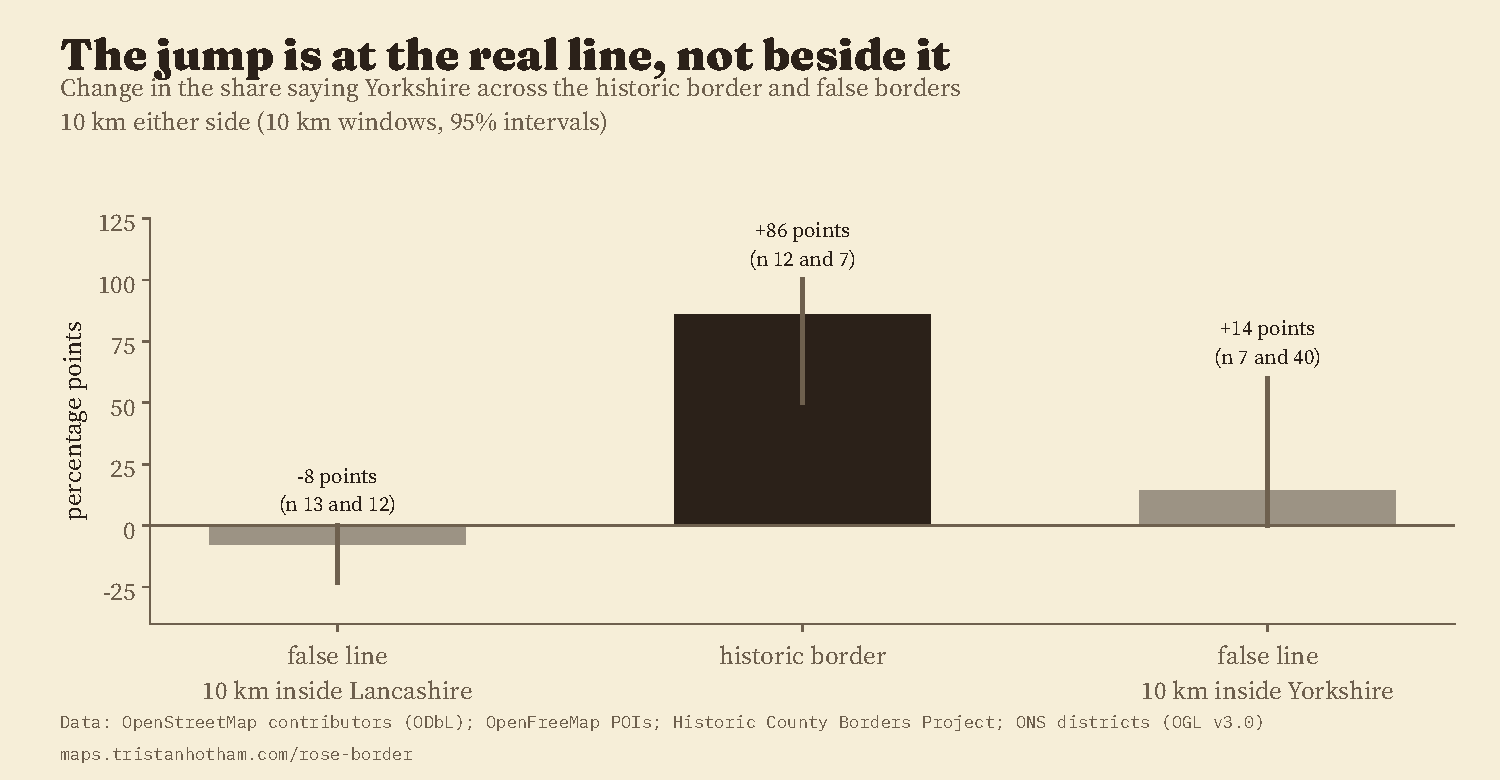
\includegraphics[width=0.8\textwidth]{f_placebo.pdf}
\caption{Placebo P1: change in the share naming Yorkshire across the historic border and across false lines 10 km into each county.}\label{fig:placebo}
\end{figure}

\begin{table}[tbp]\centering\footnotesize\caption{Placebo P1: change in the share naming Yorkshire across the real line and false lines (10 km windows either side; cluster bootstrap by 5 km cell). Below: M1b, linear probability model within 25 km.}\label{tab:placebo}\begin{tabular}{p{4.6cm}rrrrl}\toprule Line & $n$ west & $n$ east & \% west & \% east & Jump, points [95\% CI]\\\midrule
False line 10 km inside Lancashire & 13 & 12 & 7.7 & 0.0 & $-$7.7 [$-$23.1, 0.0]\\
Historic border (where it did not move) & 12 & 7 & 0.0 & 85.7 & 85.7 [50.0, 100.0]\\
False line 10 km inside Yorkshire & 7 & 40 & 85.7 & 100.0 & 14.3 [0.0, 60.0]\\
\midrule M1b: historic Yorkshire side (LPM, $n=96$, 48 clusters) & \multicolumn{5}{p{7cm}}{78.0 [44.4, 111.5] points; logit not estimable (separation)}\\
\bottomrule\end{tabular}\end{table}

\textbf{Alternative specifications.} Table~\ref{tab:robust} and Figure~\ref{fig:robust} report the 12 planned variants. The Lancashire result is stable: the rate ratio for the old Lancashire part of Greater Manchester against stayed Lancashire has an upper limit below 1 in 12 of 12 variants, and both the historic and modern coefficients of M2 for the Lancashire name exceed 1 in all 12. The Yorkshire split is not stable: the modern coefficient exceeds the historic one in 10 variants, but the order reverses when chain branches are included (a building society branch in West Craven then counts), and the model cannot be estimated with tagged features only. Bowland and West Craven contain a county-named feature only when chains or public bodies are included, so the leave-one-out split of the area into its Ribble Valley and Pendle parts adds nothing: both have none.

\begin{figure}[tbp]\centering
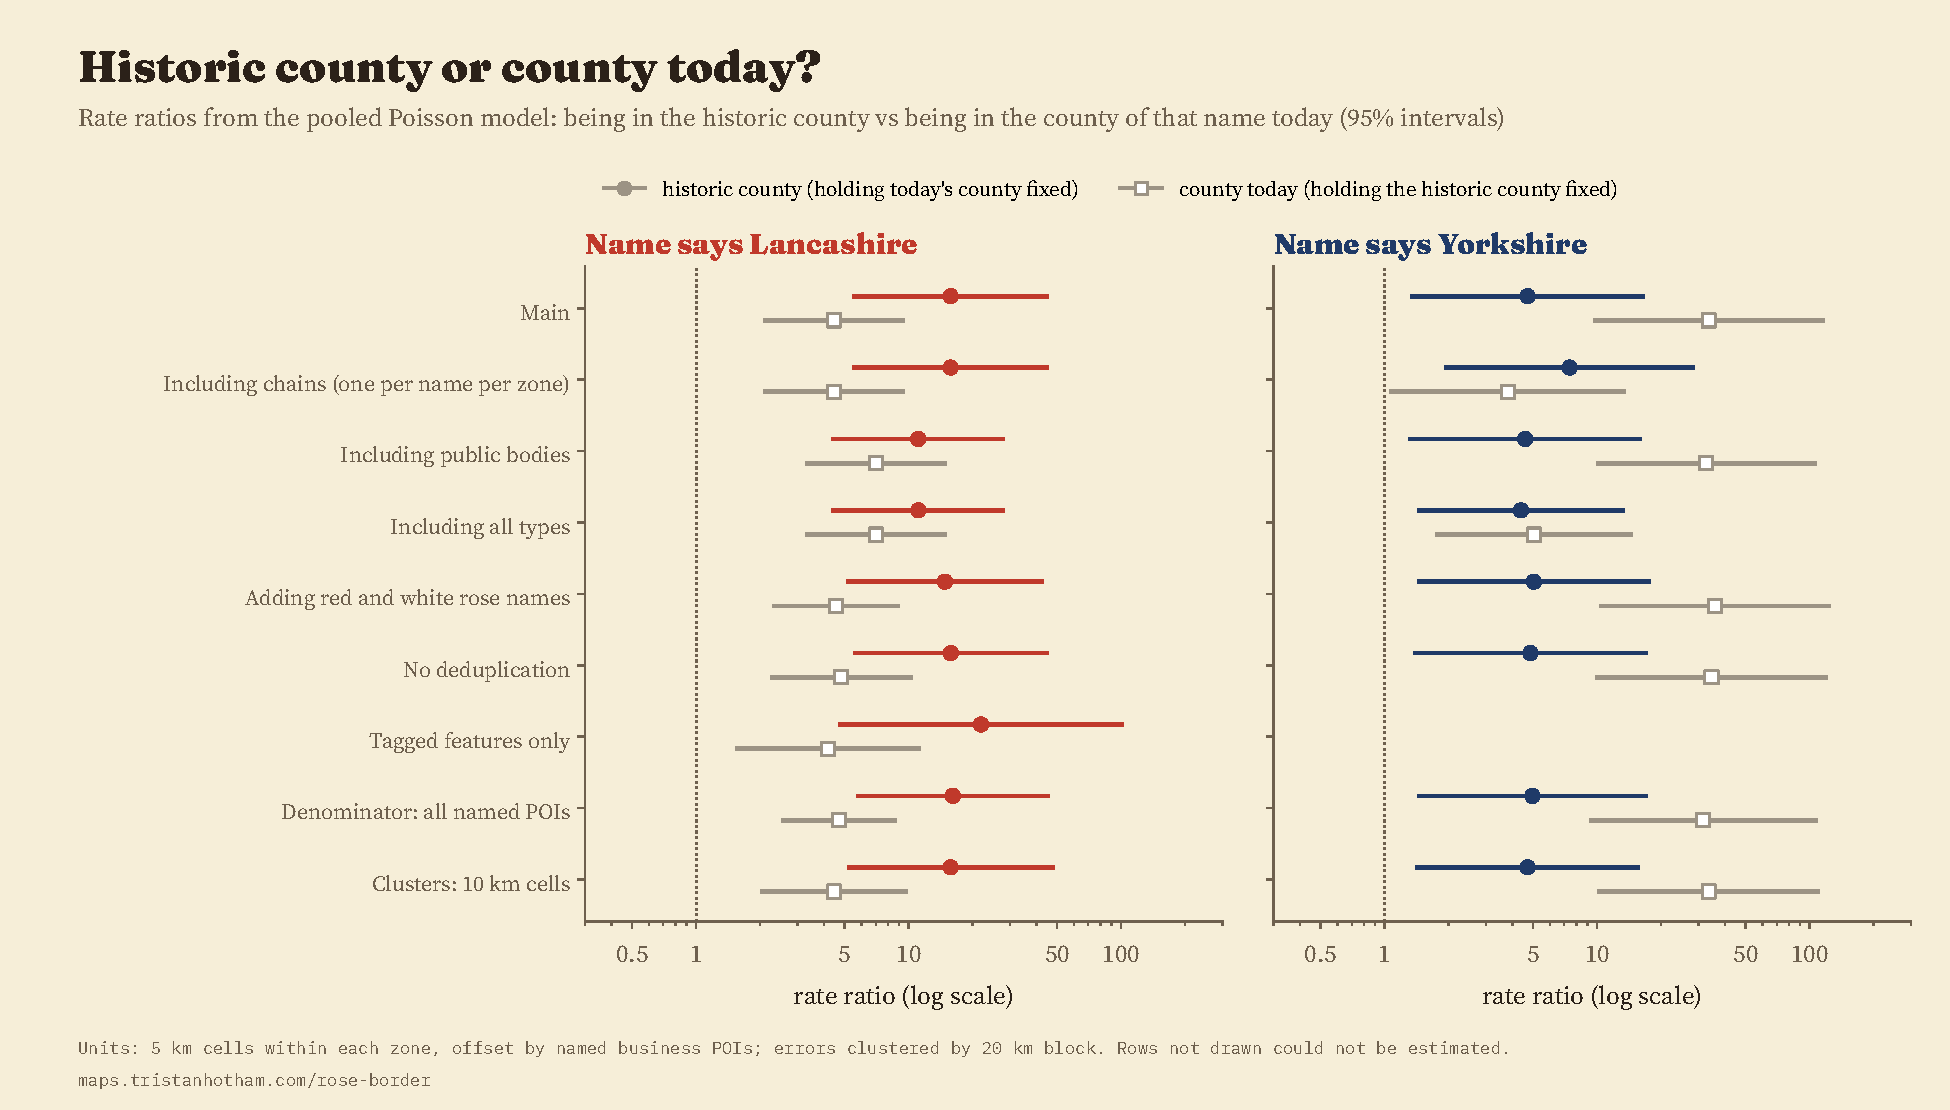
\includegraphics[width=\textwidth]{f_robust.pdf}
\caption{M2 rate ratios for the historic county and the county today under each planned check (bandwidth variants omitted: M2 does not use the band).}\label{fig:robust}
\end{figure}

\begin{table}[tbp]\centering\scriptsize\caption{Robustness. $n$: county-named features in zones. Shares: \% Yorkshire in LL / YY within the band. T\_YL: features in Bowland and West Craven. RR GM: Lancashire name, old Lancashire part of Greater Manchester vs stayed Lancashire. M2 rate ratios for the historic county (H) and the county today (M). Bandwidth changes only the band-based quantities.}\label{tab:robust}\setlength{\tabcolsep}{2.5pt}\begin{tabular}{p{3.6cm}rlrllll}\toprule Check & $n$ & LL / YY & T\_YL & RR GM [95\% CI] & Lancs. H & Lancs. M & Yorks. H / M\\\midrule
Main & 389 & 2.8 / 98.3 & 0 & 0.27 [0.15, 0.48] & 15.8 [5.6, 44.6] & 4.5 [2.1, 9.3] & 4.7 / 33.5\\
Bandwidth 10 km & 389 & 0.0 / 85.7 & 0 & 0.27 [0.15, 0.48] & 15.8 [5.6, 44.6] & 4.5 [2.1, 9.3] & 4.7 / 33.5\\
Bandwidth 15 km & 389 & 4.8 / 94.7 & 0 & 0.27 [0.15, 0.48] & 15.8 [5.6, 44.6] & 4.5 [2.1, 9.3] & 4.7 / 33.5\\
Bandwidth 40 km & 389 & 2.2 / 98.6 & 0 & 0.27 [0.15, 0.48] & 15.8 [5.6, 44.6] & 4.5 [2.1, 9.3] & 4.7 / 33.5\\
Including chains (one per name per zone) & 422 & 7.9 / 98.4 & 1 & 0.27 [0.15, 0.48] & 15.8 [5.6, 44.6] & 4.5 [2.1, 9.3] & 7.4 / 3.8\\
Including public bodies & 507 & 1.6 / 98.6 & 1 & 0.18 [0.10, 0.29] & 11.1 [4.4, 27.8] & 7.0 [3.3, 14.8] & 4.6 / 32.6\\
Including all types & 626 & 11.6 / 98.9 & 2 & 0.18 [0.10, 0.29] & 11.1 [4.4, 27.8] & 7.0 [3.3, 14.8] & 4.4 / 5.0\\
Adding red and white rose names & 449 & 2.2 / 98.5 & 0 & 0.25 [0.14, 0.43] & 14.8 [5.2, 42.2] & 4.6 [2.3, 8.9] & 5.0 / 35.9\\
No deduplication & 413 & 2.6 / 98.4 & 0 & 0.25 [0.14, 0.44] & 15.8 [5.6, 44.6] & 4.8 [2.3, 10.2] & 4.9 / 34.5\\
Tagged features only & 237 & 0.0 / 97.9 & 0 & 0.29 [0.14, 0.58] & 21.9 [4.8, 100.9] & 4.2 [1.6, 11.2] & n/a / n/a\\
Denominator: all named POIs & 389 & 2.8 / 98.3 & 0 & 0.26 [0.14, 0.45] & 16.1 [5.8, 45.1] & 4.7 [2.6, 8.6] & 5.0 / 31.6\\
Clusters: 10 km cells & 389 & 2.8 / 98.3 & 0 & 0.27 [0.15, 0.48] & 15.8 [5.2, 47.5] & 4.5 [2.0, 9.7] & 4.7 / 33.5\\
\bottomrule\end{tabular}\end{table}

\section{Discussion}\label{sec:disc}
\subsection{What the names show}
The first regularity is simple. Where the old Lancashire and Yorkshire border still separates two counties, it separates two naming worlds almost perfectly: a business near the line names itself after the county it is in. That is consistent with an identity rooted in the historic counties, but it cannot separate historic from modern identity, because along that stretch the two lines are the same.

The moved areas are where the two can be separated. Because the pre-specified primary test in Bowland and West Craven could not be estimated, the evidence here comes from the secondary comparisons in historic Lancashire outside today's Lancashire, and should be read as secondary. In Greater Manchester and Merseyside, half a century after Manchester and Liverpool left the county, Lancashire names persist at roughly a quarter (Greater Manchester) and a fifth (Merseyside) of the rate inside the county, and they are confined to the historic Lancashire side of the old Mersey and Tame boundary with Cheshire: the old Cheshire parts of the same metropolitan counties, under the same metropolitan county councils of 1974 and the same police forces today, have none. The examples include a county cricket club, a bakery and a range of trades. In the terms of \citet{zimmerbauer2017}, historic Lancashire looks ``sticky'' in the metropolitan counties: deinstitutionalised as an administration but still meaningful. At the same time, the gap from stayed Lancashire is large, and this design cannot say whether the reorganisation, the different economies and identities of the two cities, or something else accounts for it.

Further from the core, none were found. Furness and Cartmel, cut off from the rest of Lancashire by Morecambe Bay and joined to Cumbria, and Warrington and Widnes, joined to Cheshire, show no Lancashire business names. Here the data cannot say whether the name faded after 1974 or was never much used: there is no baseline from before the reform.

\subsection{What the names cannot show}
The planned primary test failed for a reason that should be reported plainly: the places moved out of Yorkshire are small and rural, and county names are rare even where they are expected. A study that wanted to know whether businesses in Barnoldswick, Earby and Saddleworth think of themselves as Yorkshire would need a richer source, such as registered company names, directories over time, or a survey. Companies House data were not reachable for this study.

Several limits apply to everything here. OpenStreetMap is volunteered and its coverage varies \citep{haklay2010}; the denominator shares that coverage, which helps, but does not guarantee that county-named businesses are mapped at the same rate as others. A name is a snapshot: firms named before 1974 cannot be separated from later ones, and nothing here dates any name. A name can follow a founder's origin, a product, or a market, as the place-branding literature would predict \citep{kavaratzis2005,pike2015}, and a regional firm's name says where it began, not where a branch is, which is why chains were set aside. Finally, the design is descriptive: it compares areas with different histories, economies and sizes and supports no causal claim about the reform.

\subsection{Relation to the literature}
The pattern adds a quantitative, open-data case to studies of regional persistence after administrative reform \citep{zimmerbauer2013,zimmerbauer2017,terlouw2016,terlouw2018}. It extends the vernacular-region tradition \citep{reed1976,zelinsky1980,liesch2015,sublett2021} from directories to OpenStreetMap and from mapping regions to testing a moved boundary. And it suggests a caution for the persistence literature in economics \citep{dell2010,becker2016,falck2012}: a sharp discontinuity at a historic border may coincide with a modern one, and the informative variation, where the two diverge, may be too thin to measure.

\section{Conclusion}\label{sec:conc}
Half a century after the 1974 reorganisation, the old Lancashire and Yorkshire border still divides business names sharply wherever it remains a county border. Where Lancashire was carved into metropolitan counties, the Lancashire name survives at a reduced rate on the historic Lancashire side and not at all on the historic Cheshire side of the same counties. Where Lancashire gave up territory to Cumbria and Cheshire, no Lancashire business names were found. And where Yorkshire gave up territory, the open map is too thin to tell which county local businesses claim. The old border shows, then, as a sharp line where it still divides counties and as a thinner Lancashire name in the metropolitan counties; whether places that left Yorkshire still name themselves after it remains open.

\section*{Data availability statement}
Data and code: Zenodo DOI https://doi.org/10.5281/zenodo.24104647. The interactive map is at \url{https://maps.tristanhotham.com/rose-border/} and the repository at \url{https://github.com/Tristan-Hotham/rose-border}. Names and points of interest: OpenStreetMap contributors (ODbL), via QLever and OpenFreeMap; historic counties: Historic County Borders Project; districts: ONS (Open Government Licence v3.0).

\section*{AI statement}
I wrote the text, with drafting and editing assistance from Claude (Anthropic), which also helped prepare the analysis code. I reviewed and checked all text and results.

\begin{thebibliography}{99}
\bibitem[Ambinakudige(2009)]{ambinakudige2009} Ambinakudige, S. (2009) Revisiting ``the South'' and ``Dixie'': delineating vernacular regions using GIS. \textit{Southeastern Geographer} 49(3), 240 to 250.
\bibitem[Becker et al.(2016)]{becker2016} Becker, S. O., Boeckh, K., Hainz, C. and Woessmann, L. (2016) The empire is dead, long live the empire! Long-run persistence of trust and corruption in the bureaucracy. \textit{Economic Journal} 126(590), 40 to 74. doi:10.1111/ecoj.12220.
\bibitem[Cameron and Miller(2015)]{cameron2015} Cameron, A. C. and Miller, D. L. (2015) A practitioner's guide to cluster-robust inference. \textit{Journal of Human Resources} 50(2), 317 to 372. doi:10.3368/jhr.50.2.317.
\bibitem[Clopper and Pearson(1934)]{clopper1934} Clopper, C. J. and Pearson, E. S. (1934) The use of confidence or fiducial limits illustrated in the case of the binomial. \textit{Biometrika} 26(4), 404 to 413. doi:10.1093/biomet/26.4.404.
\bibitem[DCLG(2013)]{dclg2013} Department for Communities and Local Government (2013) Eric Pickles: celebrate St George and England's traditional counties. News story, 23 April 2013, GOV.UK.
\bibitem[Dell(2010)]{dell2010} Dell, M. (2010) The persistent effects of Peru's mining mita. \textit{Econometrica} 78(6), 1863 to 1903. doi:10.3982/ECTA8121.
\bibitem[Falck et al.(2012)]{falck2012} Falck, O., Heblich, S., Lameli, A. and S\"udekum, J. (2012) Dialects, cultural identity, and economic exchange. \textit{Journal of Urban Economics} 72(2), 225 to 239. doi:10.1016/j.jue.2012.05.007.
\bibitem[Gao et al.(2017)]{gao2017} Gao, S., Janowicz, K., Montello, D. R., Hu, Y., Yang, J.-A., McKenzie, G., Ju, Y., Gong, L., Adams, B. and Yan, B. (2017) A data-synthesis-driven method for detecting and extracting vague cognitive regions. \textit{International Journal of Geographical Information Science} 31(6), 1245 to 1271. doi:10.1080/13658816.2016.1273357.
\bibitem[Garwood(1936)]{garwood1936} Garwood, F. (1936) Fiducial limits for the Poisson distribution. \textit{Biometrika} 28(3/4), 437 to 442.
\bibitem[Giovannini(2016)]{giovannini2016} Giovannini, A. (2016) Towards a ``new English regionalism'' in the North? The case of Yorkshire First. \textit{Political Quarterly} 87(4), 590 to 600. doi:10.1111/1467-923X.12279.
\bibitem[Goodchild(2007)]{goodchild2007} Goodchild, M. F. (2007) Citizens as sensors: the world of volunteered geography. \textit{GeoJournal} 69(4), 211 to 221. doi:10.1007/s10708-007-9111-y.
\bibitem[Gulley(1990)]{gulley1990} Gulley, H. E. (1990) Southern nationalism on the landscape: county names in former Confederate states. \textit{Names} 38(3), 231 to 240. doi:10.1179/nam.1990.38.3.231.
\bibitem[Haklay(2010)]{haklay2010} Haklay, M. (2010) How good is volunteered geographical information? A comparative study of OpenStreetMap and Ordnance Survey datasets. \textit{Environment and Planning B} 37(4), 682 to 703. doi:10.1068/b35097.
\bibitem[Hansard(1974)]{hansard1974} House of Commons (1974) County boundary signs. Written answer, HC Deb 20 June 1974, vol. 875, col. 237W.
\bibitem[HCBP(2024)]{hcbp2024} Historic County Borders Project (2024) UK Definition A county border vector data (simplified). Historic Counties Trust. Accessed 2026. \url{https://www.county-borders.co.uk}.
\bibitem[Hollenstein and Purves(2010)]{hollenstein2010} Hollenstein, L. and Purves, R. (2010) Exploring place through user-generated content: using Flickr tags to describe city cores. \textit{Journal of Spatial Information Science} 2010(1), 21 to 48.
\bibitem[Jones and MacLeod(2004)]{jones2004} Jones, M. and MacLeod, G. (2004) Regional spaces, spaces of regionalism: territory, insurgent politics and the English question. \textit{Transactions of the Institute of British Geographers} 29(4), 433 to 452.
\bibitem[Kavaratzis(2004)]{kavaratzis2004} Kavaratzis, M. (2004) From city marketing to city branding: towards a theoretical framework for developing city brands. \textit{Place Branding} 1(1), 58 to 73. doi:10.1057/palgrave.pb.5990005.
\bibitem[Kavaratzis and Ashworth(2005)]{kavaratzis2005} Kavaratzis, M. and Ashworth, G. J. (2005) City branding: an effective assertion of identity or a transitory marketing trick? \textit{Tijdschrift voor Economische en Sociale Geografie} 96(5), 506 to 514. doi:10.1111/j.1467-9663.2005.00482.x.
\bibitem[Keele and Titiunik(2015)]{keele2015} Keele, L. J. and Titiunik, R. (2015) Geographic boundaries as regression discontinuities. \textit{Political Analysis} 23(1), 127 to 155. doi:10.1093/pan/mpu014.
\bibitem[Leach et al.(2016)]{leach2016} Leach, H., Watson, K. and Gnevsheva, K. (2016) Perceptual dialectology in northern England: accent recognition, geographical proximity and cultural prominence. \textit{Journal of Sociolinguistics} 20(2), 192 to 211. doi:10.1111/josl.12178.
\bibitem[LGA(1972)]{lga1972} Local Government Act 1972 (c. 70). London: HMSO. In force 1 April 1974.
\bibitem[Liesch et al.(2015)]{liesch2015} Liesch, M., Dunklee, L. M., Legg, R. J., Feig, A. D. and Krause, A. J. (2015) Use of business-naming practices to delineate vernacular regions: a Michigan example. \textit{Journal of Geography} 114(5), 188 to 196. doi:10.1080/00221341.2014.965187.
\bibitem[ONS(2023)]{ons2023} Office for National Statistics (2023) Local Authority Districts (December 2023) boundaries UK, generalised clipped. Open Government Licence v3.0.
\bibitem[OpenFreeMap(2026)]{openfreemap2026} OpenFreeMap (2026) Planet vector tiles, OpenMapTiles schema, zoom 14. \url{https://openfreemap.org}. Data: OpenStreetMap contributors, ODbL.
\bibitem[OpenStreetMap contributors(2026)]{osm2026} OpenStreetMap contributors (2026) Planet data queried through QLever (osm-planet). Open Database Licence.
\bibitem[Paasi(1986)]{paasi1986} Paasi, A. (1986) The institutionalization of regions: a theoretical framework for understanding the emergence of regions and the constitution of regional identity. \textit{Fennia} 164, 105 to 146. doi:10.11143/9052.
\bibitem[Paasi(2003)]{paasi2003} Paasi, A. (2003) Region and place: regional identity in question. \textit{Progress in Human Geography} 27(4), 475 to 485. doi:10.1191/0309132503ph439pr.
\bibitem[Pike(2015)]{pike2015} Pike, A. (2015) \textit{Origination: The Geographies of Brands and Branding}. Chichester: Wiley-Blackwell.
\bibitem[Reed(1976)]{reed1976} Reed, J. S. (1976) The heart of Dixie: an essay in folk geography. \textit{Social Forces} 54(4), 925 to 939.
\bibitem[Royal Commission(1969)]{rc1969} Royal Commission on Local Government in England 1966 to 1969 (1969) \textit{Report} (Chairman: Lord Redcliffe-Maud). Cmnd 4040. London: HMSO.
\bibitem[Russell(2004)]{russell2004} Russell, D. (2004) \textit{Looking North: Northern England and the National Imagination}. Manchester: Manchester University Press.
\bibitem[Sublett(2021)]{sublett2021} Sublett, M. D. (2021) Corn Belt as an enterprise-naming custom in the United States. \textit{Names} 69(4), 1 to 12. doi:10.5195/names.2021.2254.
\bibitem[Terlouw(2016)]{terlouw2016} Terlouw, K. (2016) Territorial changes and changing identities: how spatial identities are used in the up-scaling of local government in the Netherlands. \textit{Local Government Studies} 42(6), 938 to 957. doi:10.1080/03003930.2016.1186652.
\bibitem[Terlouw(2018)]{terlouw2018} Terlouw, K. (2018) Transforming identity discourses to promote local interests during municipal amalgamations. \textit{GeoJournal} 83, 525 to 543. doi:10.1007/s10708-017-9785-8.
\bibitem[Wales(2006)]{wales2006} Wales, K. (2006) \textit{Northern English: A Social and Cultural History}. Cambridge: Cambridge University Press.
\bibitem[Wilson(1927)]{wilson1927} Wilson, E. B. (1927) Probable inference, the law of succession, and statistical inference. \textit{Journal of the American Statistical Association} 22(158), 209 to 212. doi:10.2307/2276774.
\bibitem[Zelinsky(1980)]{zelinsky1980} Zelinsky, W. (1980) North America's vernacular regions. \textit{Annals of the Association of American Geographers} 70(1), 1 to 16.
\bibitem[Zimmerbauer and Paasi(2013)]{zimmerbauer2013} Zimmerbauer, K. and Paasi, A. (2013) When old and new regionalism collide: deinstitutionalization of regions and resistance identity in municipality amalgamations. \textit{Journal of Rural Studies} 30, 31 to 40. doi:10.1016/j.jrurstud.2012.11.004.
\bibitem[Zimmerbauer et al.(2017)]{zimmerbauer2017} Zimmerbauer, K., Riukulehto, S. and Suutari, T. (2017) Killing the regional Leviathan? Deinstitutionalization and stickiness of regions. \textit{International Journal of Urban and Regional Research} 41(4), 676 to 693. doi:10.1111/1468-2427.12547.
\end{thebibliography}

\appendix
\section{Appendix: data construction}
\begin{table}[tbp]\centering\small\caption{From the name file to the main sample.}\label{tab:flow}\begin{tabular}{lr}\toprule Step & Number\\\midrule
Rows in the OSM name file & 7,500\\
with a Lancashire, Yorkshire or rose word & 2,693\\
\quad less: highway & $-$889\\
\quad less: line (railway, canal, path) & $-$757\\
\quad less: street name & $-$37\\
\quad less: route or stop & $-$29\\
\quad less: landmark or natural feature & $-$7\\
\quad less: administrative area & $-$7\\
\quad less: car park & $-$7\\
\quad less: product or breed & $-$4\\
\quad less: surname & $-$2\\
\quad less: duplicate & $-$1\\
\quad less: duplicates (same name within 300 m) & $-$39\\\midrule
Kept & 914\\
\quad private & 491\\
\quad chain & 296\\
\quad public & 127\\
Outside the study zones & 205\\
Main sample: private, county word, in zones & 389 (77 Lancashire, 312 Yorkshire)\\
\bottomrule\end{tabular}\end{table}

\textbf{Decisions made by hand} (\texttt{code/overrides.csv}). Dropped as routes or stops: bus route and stop relations named after shopping centres and streets (``White Rose Centre'', ``Yorkshire Television Studios''), long-distance paths and cycle routes, railway lines and stations. Dropped as administrative areas: boundary relations named Lancashire, West Lancashire, West Riding of Yorkshire, West Yorkshire and the Yorkshire Dales National Park. Dropped as landmarks: memorials to the Lancashire Fusiliers and the Loyal North Lancashire Regiment, a monument to Lancashire dialect poets, a moor and a community forest. Dropped: car parks of named sites; a golf club mapped twice more than 300 m apart; a car dealer whose name is its founders' surname. Retyped: regional broadcasters, council offices, a probation company, NHS units and a further education college as public; private hospitals, private schools and colleges, a hospice charity and a water-ski club as private. No feature was dropped or retyped by reference to its zone or to the outcome.

\textbf{Software.} Python 3 with pandas, numpy, geopandas, shapely, pyproj, statsmodels, scipy, mapbox-vector-tile and matplotlib; xelatex. All code is in the repository and the data and code archive.

\end{document}
